\section{Feature representation}
\subsection{Handcrafted Action Features}
\begin{frame}{Handcrafted Action Features (RGB)}
    \begin{enumerate}
        \item<1-> Spatiotemporal volume-based action representation methods (\href{https://web.cse.ohio-state.edu/~davis.1719/CVL/Research/MHI/mhi.html}{motion history image, motion energy image}) \cite{li2011human}.
              \only<1>{
                  \begin{figure}[htp]
                      \centering
                      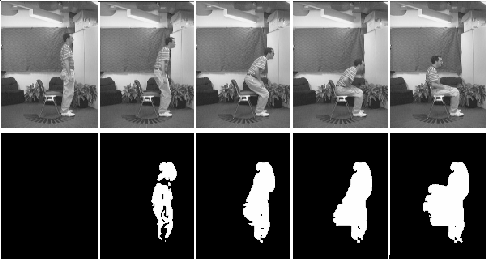
\includegraphics[height=2.25cm, width=10cm]{topics/201010-zhang2019comprehensive/assets/img/mei.png}
                      \caption{Motion history image}
                  \end{figure}
                  \begin{figure}[htp]
                      \centering
                      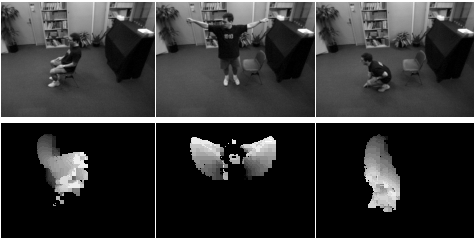
\includegraphics[height=2.25cm, width=10cm]{topics/201010-zhang2019comprehensive/assets/img/mhi.png}
                      \caption{Motion energy image}
                  \end{figure}
              }
              % [Global features] The camera is fixed  -> background subtraction techniques
              % -> shape information (silhouettes and contours) -> key template matrix -> matching
        \item<2-> STIP-based methods (Feature descriptors: SIFT, HOG) \cite{nguyen2014stap}, \cite{dalal2005histograms}.
              \only<2>{
                  \begin{figure}[htp]
                      \centering
                      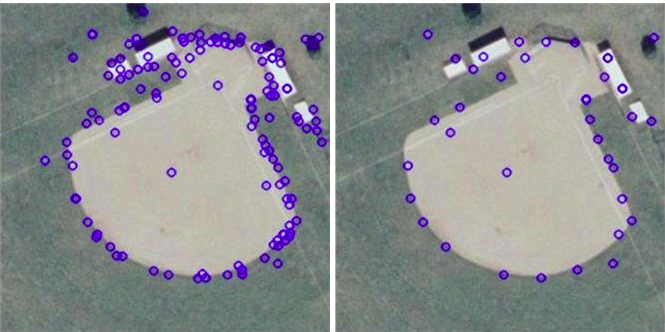
\includegraphics[width=0.6\textwidth]{topics/201010-zhang2019comprehensive/assets/img/sift.png}
                      \caption{Scale-invariance feature transform}
                  \end{figure}
              }
              % [Local features] key region of movement change.
        \item<3-> Action representation methods based on the trajectory of skeleton joints.
              % tracking path of key points or the joints in the human skeleton
              \only<3>{
                  \begin{figure}[htp]
                      \centering
                      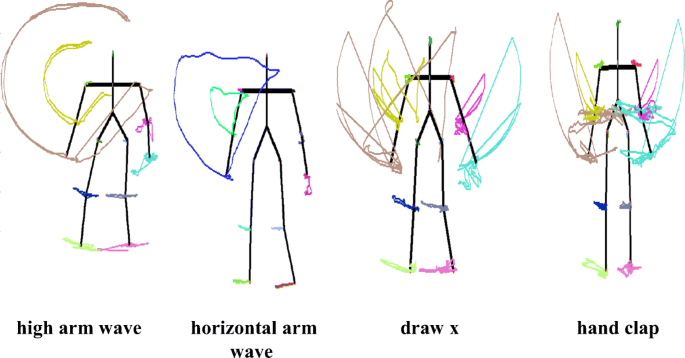
\includegraphics[width=0.5\textwidth]{topics/201010-zhang2019comprehensive/assets/img/joins-trajectory.png}
                      \caption{Scale-invariance feature transform}
                  \end{figure}
              }
    \end{enumerate}
\end{frame}

\subsection{Methods Based on Deep Learning}
\begin{frame}{Methods Based on Deep Learning}
    \begin{itemize}
        \item In recent years, the application of deep learning to computer vision has received considerable attention.
        \item Many deep learning-based action representation methods have been proposed in the field of human action recognition
              \begin{enumerate}
                  \item 3D convolutional networks.
                  \item Two-stream convolutional networks \cite{simonyan2014two}.
                  \item Long short-term memory (LSTM).
              \end{enumerate}
    \end{itemize}
\end{frame}

\begin{frame}{3D convolutional networks}
    \begin{figure}[htp]
        \centering
        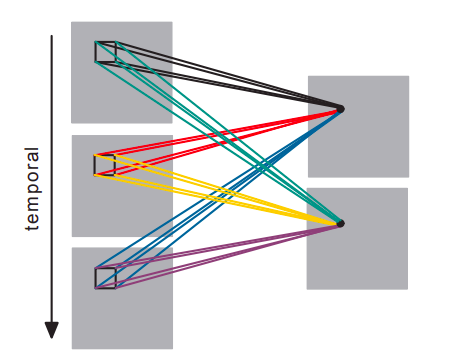
\includegraphics[width=0.5\textwidth]{topics/201010-zhang2019comprehensive/assets/img/3d-cnn.png}
        \caption{3D convolutional networks}
    \end{figure}
\end{frame}

\begin{frame}{Two-stream convolutional networks}
    \begin{figure}[htp]
        \centering
        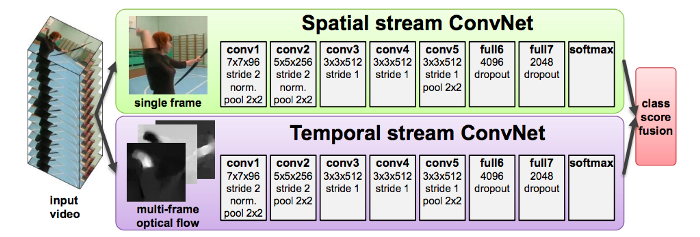
\includegraphics[width=\textwidth]{topics/201010-zhang2019comprehensive/assets/img/2-stream-cnn.png}
        \caption{Two-stream convolutional networks}
    \end{figure}
\end{frame}

\begin{frame}[allowframebreaks]
    \frametitle{Long short-term memory (LSTM)}
    \begin{figure}[htp]
        \centering
        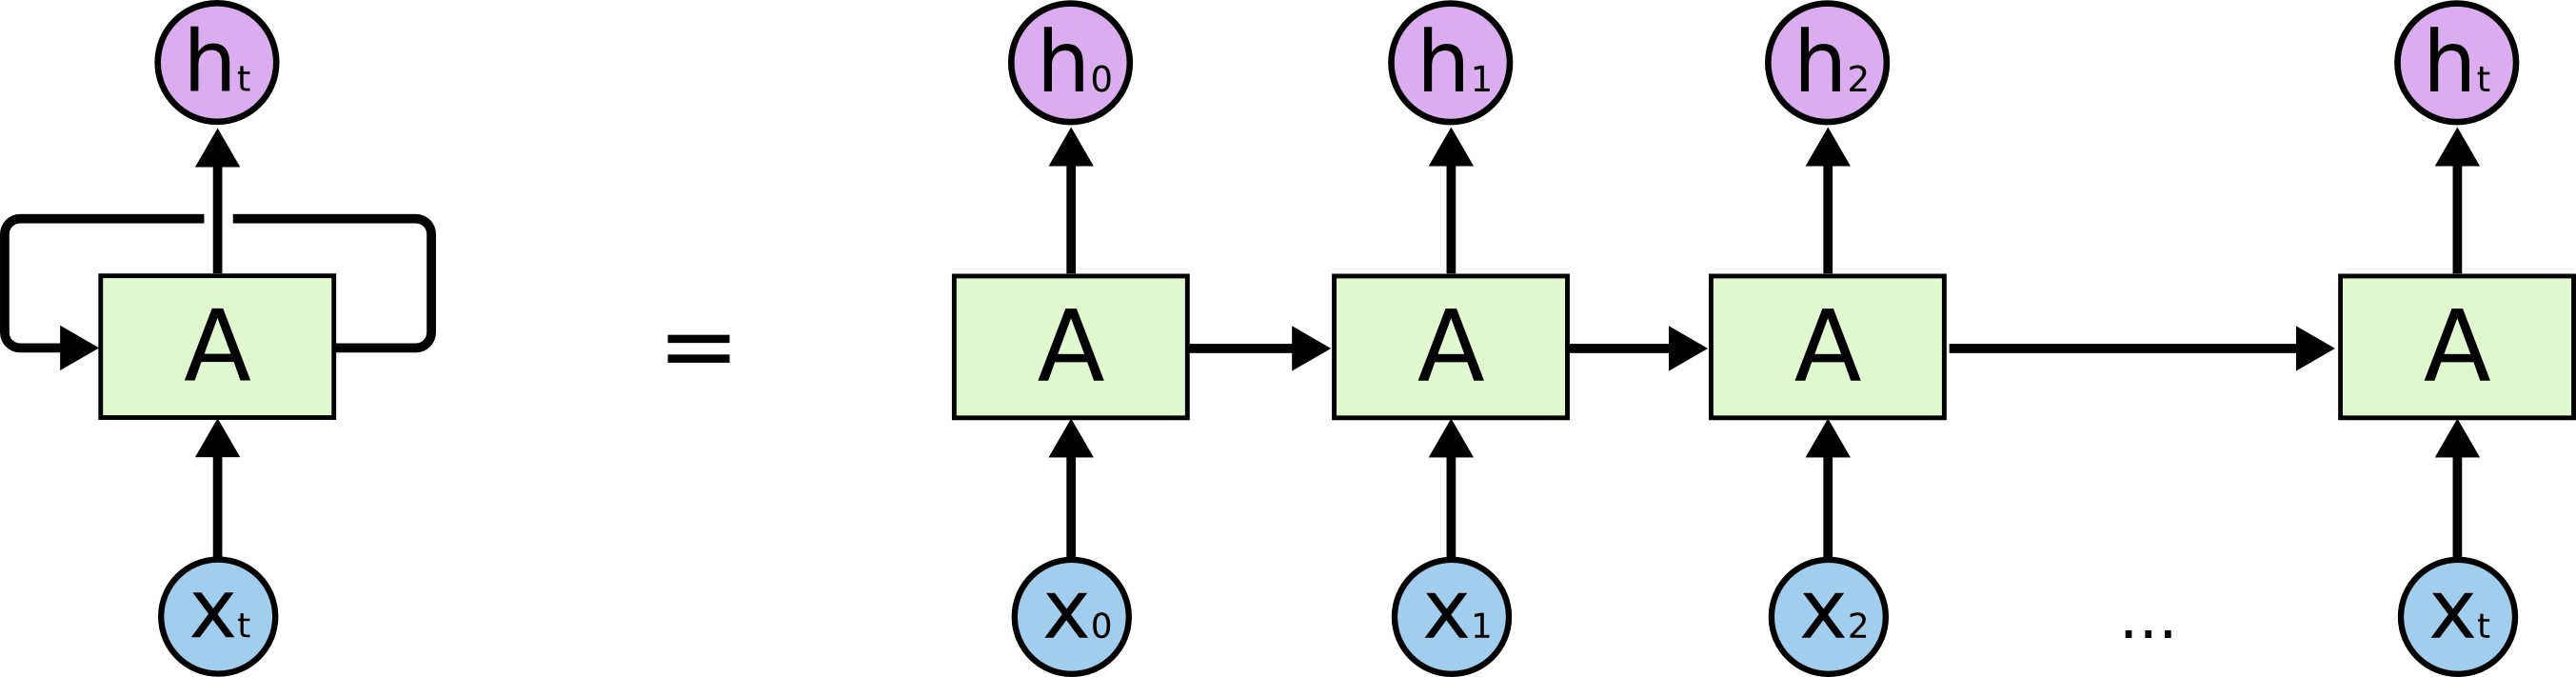
\includegraphics[width=\textwidth]{topics/201010-zhang2019comprehensive/assets/img/RNN-unrolled.png}
        \caption{RNN}
    \end{figure}
    \begin{figure}[htp]
        \centering
        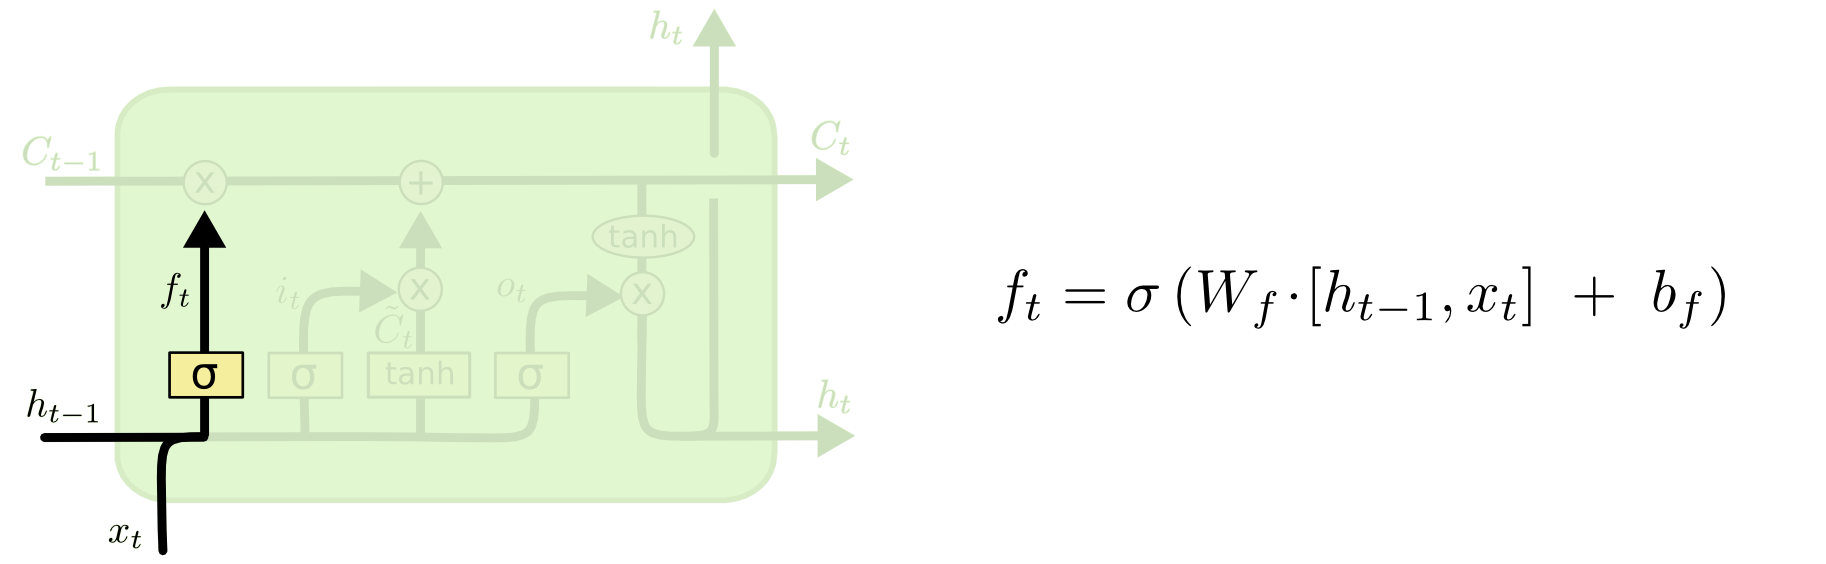
\includegraphics[width=\textwidth]{topics/201010-zhang2019comprehensive/assets/img/LSTM-1.png}
        \caption{Forget gate layer}
    \end{figure}
    \begin{figure}[htp]
        \centering
        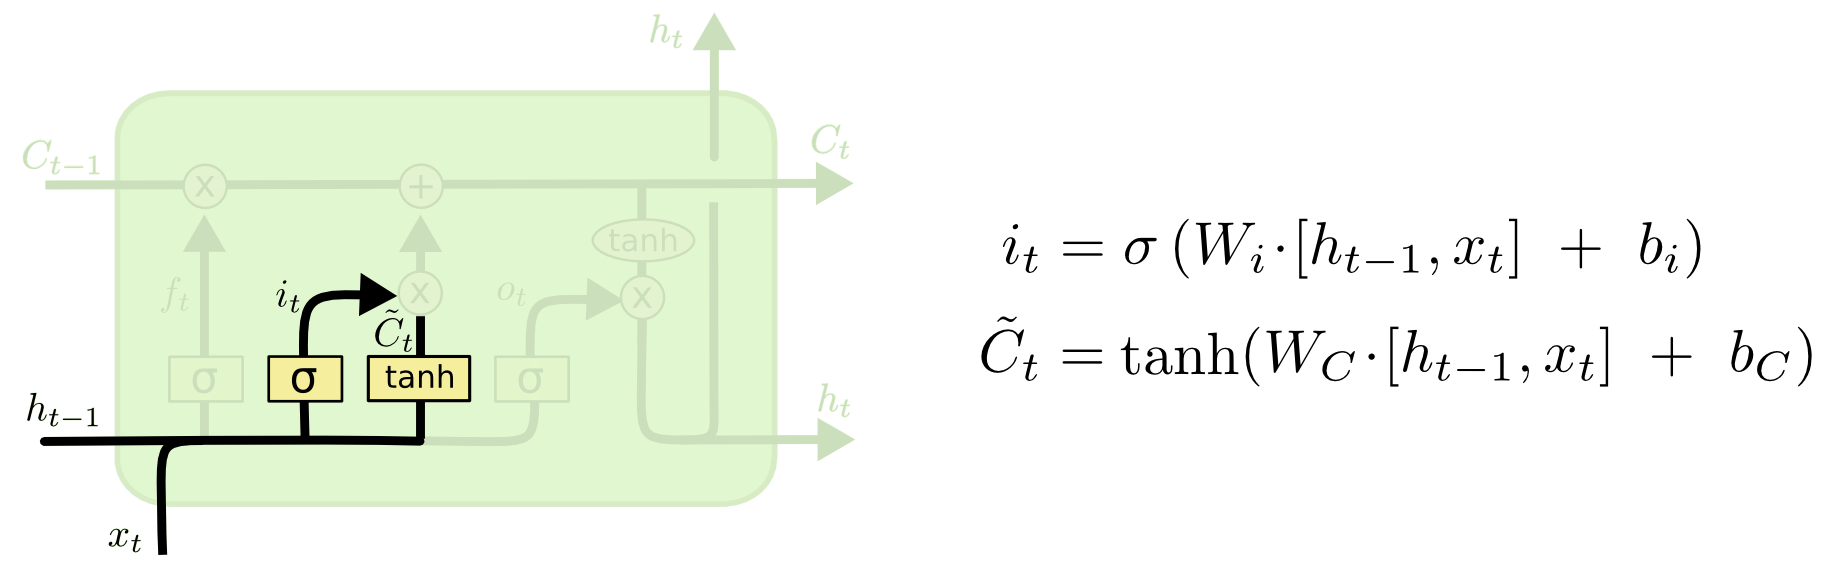
\includegraphics[width=\textwidth]{topics/201010-zhang2019comprehensive/assets/img/LSTM-2.png}
        \caption{Input gate layer}
    \end{figure}
    \begin{figure}[htp]
        \centering
        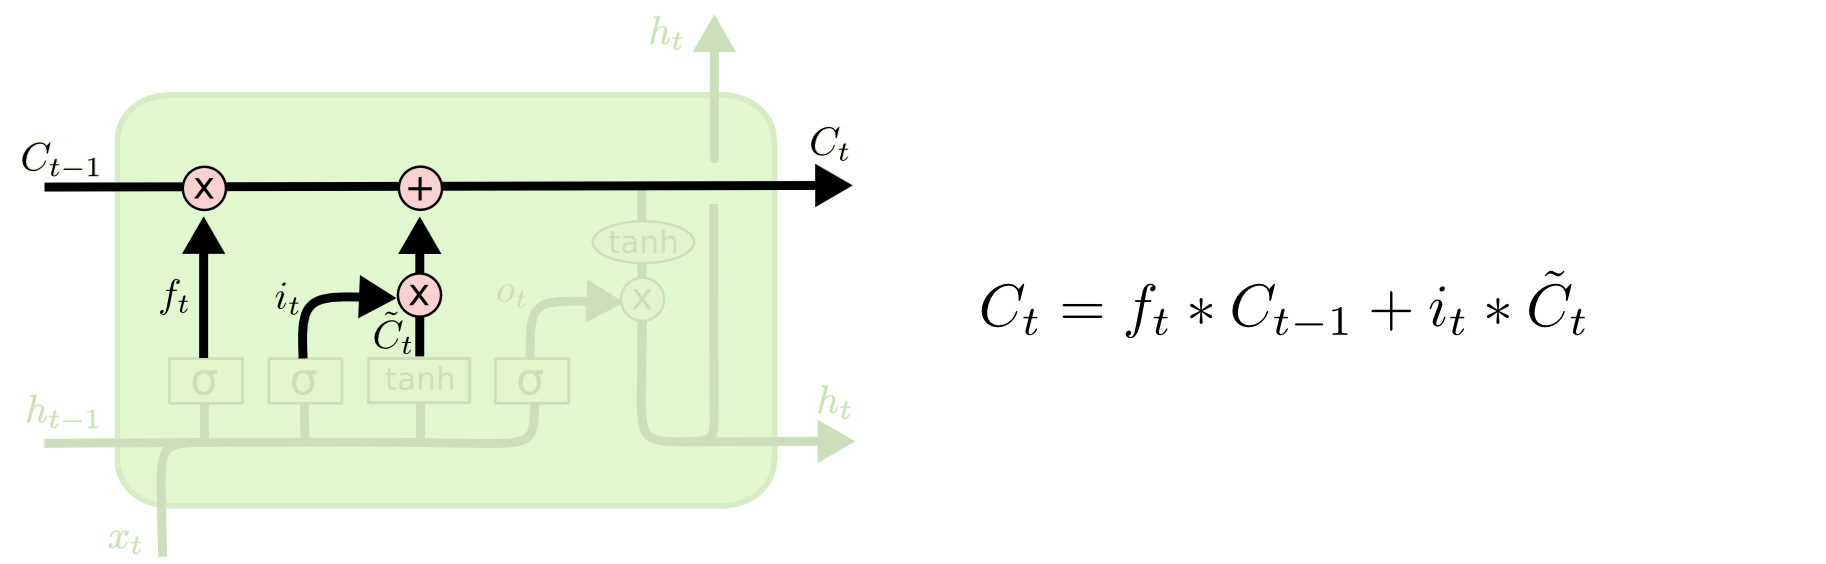
\includegraphics[width=\textwidth]{topics/201010-zhang2019comprehensive/assets/img/LSTM-3.png}
        \caption{Update gate layer}
    \end{figure}
    \begin{figure}[htp]
        \centering
        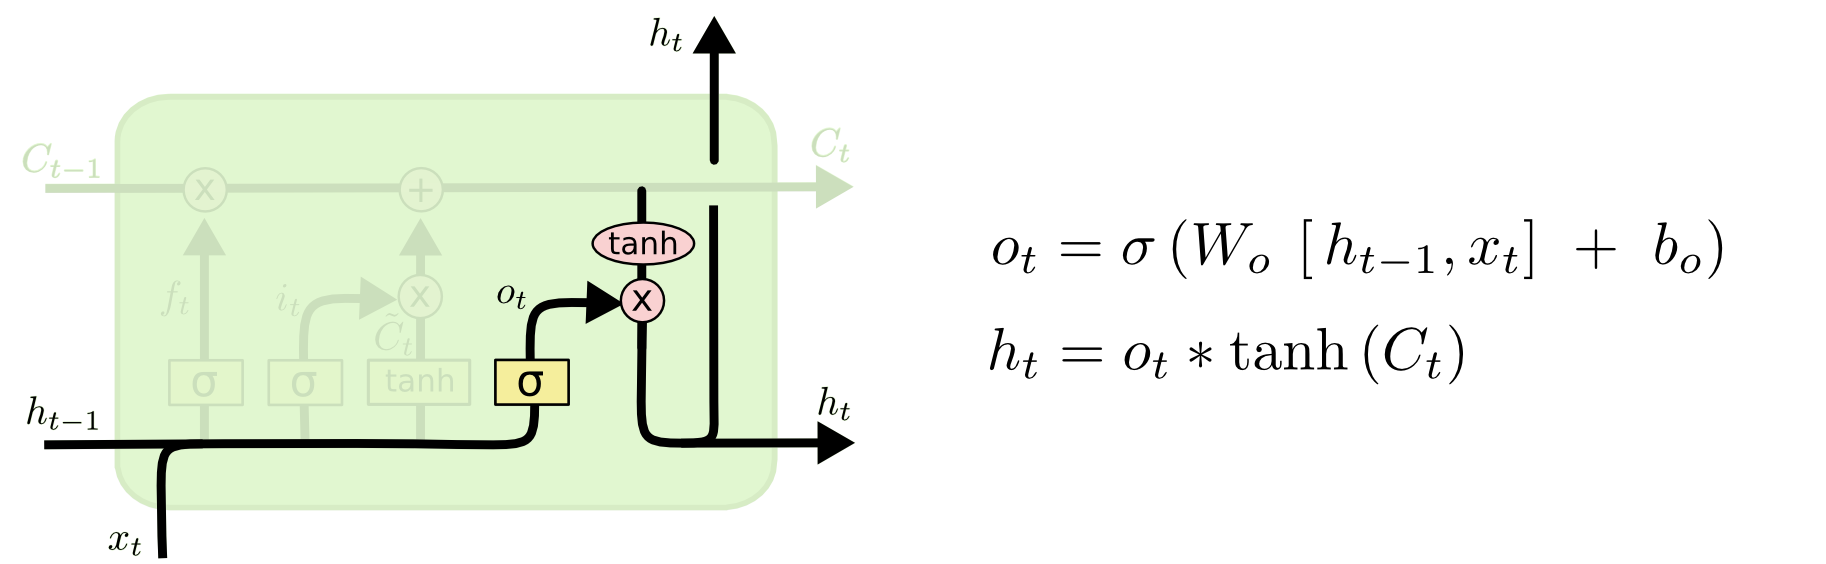
\includegraphics[width=\textwidth]{topics/201010-zhang2019comprehensive/assets/img/LSTM-4.png}
        \caption{Output gate layer}
    \end{figure}
\end{frame}